\documentclass[a4paper, 11pt, twoside]{article}
\usepackage{amssymb}
\usepackage{amsmath}
\usepackage{graphicx}
\begin{document}
\title{MATH6222 week 5 lecture 12}
\author{Rui Qiu}
\date{2017-03-20}

\maketitle

Midterm on April 21st.\\

\textbf{4 Questions:}
\begin{enumerate}
	\item Is $\mathbb{N}$ smallest infinite set?
	\item Other sizes besides $\mathbb{N}$ and $\mathbb{R}$?
	\item What is a real number?
	\item Is our definition of $\leq$ sensible?
\end{enumerate}

\paragraph{Face:} Every real number has a unique decimal expansion if we disallow expansions that ends in an infinite sequence of $9$'s.

\[12.999\dots\]
\[13.000\dots\]

Let's call such an expansion "good".\\

\paragraph{Theorem:} $|\mathbb{N}| < |\mathbb{R}|$.

\paragraph{Proof:} Suppose $\exists$ bijection $f:\mathbb{N}\to\mathbb{R}$.
\[1\to \dots\dots . a_{11}a_{12}a_{13}\dots\]
\[2\to \dots\dots . a_{21}a_{22}a_{23}\dots\]
\[3\to \dots\dots . a_{31}a_{32}a_{33}\dots\]

Let's produce a real number \textbf{not} in the image of $f$.

Let's define $b_1, b_2, b_3, \dots$ by rule:

\[b_i:=\begin{cases}
	4, &\text{ if } a_{ii}\not=4;\\
	5, &\text{ if } a_{ii}=4.
\end{cases}
\]

Claim that the real number $\dots\dots. b_1b_2b_3\dots$ is not in image of $f$.

Same diagonal argument as before.\\

Is $\mathbb{R}^2\to \mathbb{R}$?

$(0,1)\times(0,1)\to (0,1)$

$.x_1x_2x_3x_4\dots$

$.y_1y_2y_3y_4\dots$

$\to .x_1y_1x_2y_2x_3y_3x_4y_4\dots$

Check injective and surjective.\\

Injectivity:

$(.x_1x_2x_3\dots,.y_1y_2y_3\dots)\to .x_1y_1x_2y_2x_3y_3\dots x_i$

$(.x_1'x_2'x_3'\dots,.y_1'y_2'y_3'\dots)\to .x_1'y_1'x_2'y_2'x_3'y_3'\dots x_i'$

For some $i$, either $x_i\not=x_i'$ or $y_i\not=y_i'$\\

Surjectivity:

Think about $.1919191919\dots$, not surjective.

\textbf{Question:} Does $|A|\leq|B|$ and $|B|\leq|A| \implies |A|=|B|?$

This is to say, $\exists$ injection $A\to B$, $\exists$ injection $B\to A$, but $exists$ bijection $A\to B$?

This is true. Pretty obvious for finite sets, but for infinite sets? (It is true as well)\\

\paragraph{Corollary:} $|(0,1)\times(0,1)|=|(0,1)|$.

\paragraph{Theorem:} $|\mathbb{N}| < |S|$ where $S$ is the set of $0,1$ sequences.\\

I claim $S\to 2^{\mathbb{N}}:=\{\text{subsets of }\mathbb{N}\}$\\

\[01100010\dots \to \{2,3,7,\dots\}\]
\[10110010\dots \to \{1,3,4,7,\dots\}\]

\paragraph{Theorem:} For any set $S$, we claim $|S|<|2^{S}|$.\\

\paragraph{Corollary:} $|\mathbb{N}|<|2^{\mathbb{N}}|<|2^{2^{\mathbb{N}}}|<\dots$

\paragraph{Proof:}\ \\

Injection: $S\to 2^{S}$.

$x\to \{x\} (\subseteq S)$\\

Bijection:

Suppose $\exists$ bijection $f:S\to 2^{S}$

We want to produce a subset $T\subseteq S$ such that $T$ is not in the image of $f$.

Define $T$ as follows:

\[x \in T \iff x\not\in f(x)\]

It follow that $ T\not = f(x)$ for any $x\in S$. Done.\\

We have 2 sets from $A\to B$ 

$f:A\to B$ and $g: B\to A$

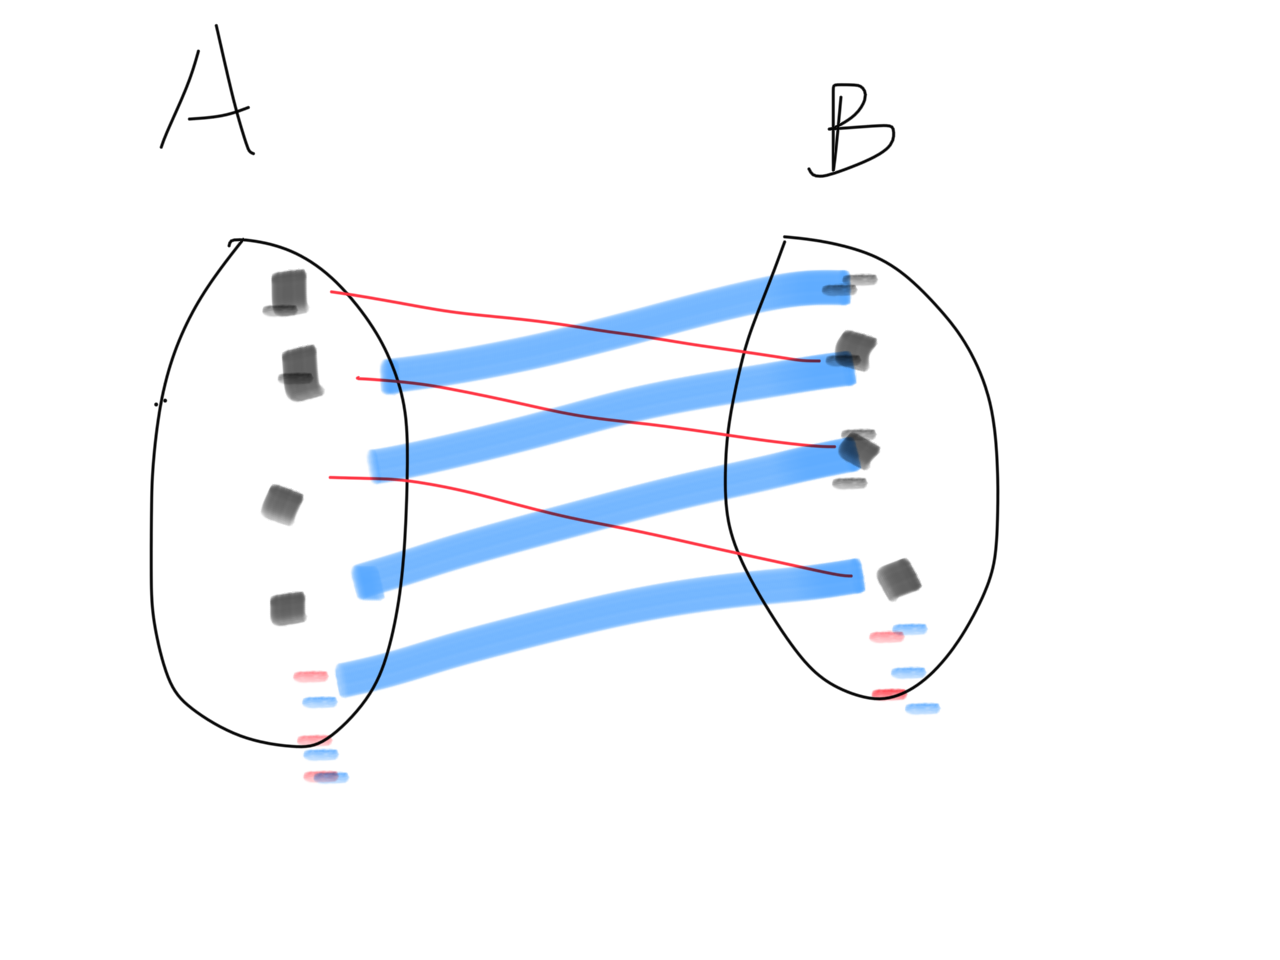
\includegraphics[width=\textwidth]{images/AB}
\end{document}

